\section{Discovery of Extremal Microstructure Families}
\label{sec:discovery}
Microstructures can exhibit remarkable physical properties that extend beyond the properties of their constituent materials.
Many microstructure types have been developed to demonstrate applications
in mechanics~\citep{milton1995,kadic2012practicability,meza2014strong,zheng2014ultralight,li2016mechanical,wang2016lightweight},
acoustics~\citep{fang2006ultrasonic,li2009experimental}, 
and electromagnetics~\citep{schurig2006metamaterial,shalaev2007optical}.
These microstructures are typically designed by domain experts using time and labor intensive manual processes. These designs are often programmable in the sense that they have a small number of parameters to generate a family of geometries. A given microstructure family can be tested by performing simulations or experimental measurements on a set of samples drawn from it. The mapping between parameters and physical properties discovered in this testing process helps uncover the underlying design principles that drive these correspondences.
In practical applications, mapping the parameter space also allows for the selection of a family member that has a desired tradeoff of physical properties~\citep{gibson1982mechanics}.
Unfortunately, it is rare for manually designed microstructure families to reach extremal properties. This is because the space of possible microstructure designs is combinatorial and therefore impossible to explore exhaustively.
One common approach to bypass this design challenge is to use computational methods,
such as topology optimization~\citep{sigmund1994materials,vogiatzis2017topology}, with a computer simulation in their inner loop to find a microstructure with a desired tradeoff of physical properties.
Unfortunately, constructing parametric models from these optimized structures has heretofore required further expertise and manual design effort~\citep{clausen2015topology}.
In contrast to previous work, we present the first computational method to automatically explore the space of microstructure designs and discover parametric families optimized for competing properties.

While our methodology is not limited to specific physical properties, this study applied our method to design of mechanical microstructures. Specifically, we set our algorithm to search for a particularly interesting type of mechanical microstructures: auxetic materials, which have a negative Poisson's ratio.
These materials have the unusual property of becoming laterally thinner under axial compression.
2D auxetic structures are well understood due to their relatively simple geometry such as reentrant structures~\citep{sigmund1994materials,lakes1987foam},
chiral structures~\citep{prall1997properties,ha2016chiral}
and rotating mechanisms~\citep{babaee20133d,buckmann2014three}.
Generalizing existing 2D structures to 3D is challenging since a naive arrangement of 2D mechanisms often results in orthotropic or other anisotropic structures with low shear resistance. Such structures will prefer shearing deformation when the load is not aligned well with the auxetic direction. Additionally, since Poisson's ratio for orthotropic structures is unbounded, orthotropic auxetic structures are much easier to find than isotropic ones18. Lakes fabricated and tested the first isotropic 3D auxetic structure13. However, designing manufacturable 3D auxetic structures remains a challenging task due to its complexity.
Only a handful of 3D design patterns have been fabricated and measured~\citep{andreassen2014design,saxena2016three}.
This study led to the discovery of five families with negative Poisson's ratio and tunable shear resistance.
\subsection{Discovery Pipeline}
\begin{figure}
	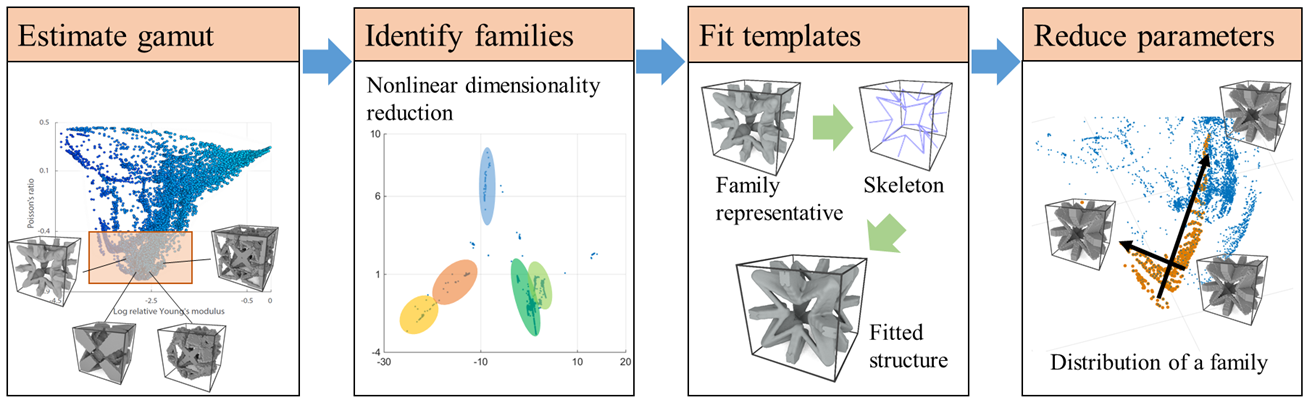
\includegraphics[width=\textwidth]{images/discoveryPipeline.png}
	\caption{A computational process for discovery of extremal microstructure families. Given a set of physical properties and design constraints, we estimate the material property gamut using stochastic sampling and topology optimization. Structures near the gamut boundary are grouped into families using nonlinear dimensionality reduction. A representative from each family is fitted with a template represented as a skeleton. Beams are placed on the skeleton edges with optimized parameters to fit the original structure. Structure variations with the same topology can be generated by varying the beam parameters. Finally, reduced template parameters are computed to reveal domain-specific design principles. }
	\label{fig:discovery}
\end{figure}
Our discovery pipeline has four steps (Figure~\ref{fig:discovery}). The first step estimates the material property gamut, which is the range of material properties achievable by the microstructures. Here a microstructure is defined on a 3D regular grid composed of hexahedral voxels. The design space includes all possible material assignments to the voxels.
Since exhaustively simulating all possible microstructures is impractical, this step computes a set of sample microstructures using methods outlined in Section~\ref{sec:sampling}.
The topology optimization stage pushes structures past the explored gamut boundary along gradient directions. The stochastic stage introduces discrete changes to escape local optima.

In the second step, common geometric traits are identified among microstructures near the gamut boundary. Geometrically similar structures are grouped into families using nonlinear dimensionality reduction (NLDR). Isomap~\citep{tenenbaum2000global} is used as the reduction method because it can discover long sequences of related structures while keeping distant points separated. The effectiveness of NLDR depends on the distance metric that measures geometric difference. A smoothed Euclidean norm is chosen for robustness (Supplementary Fig. 1). NLDR outputs an embedding of the microstructures in a low-dimensional space where similar structures are closely packed.
Microstructures in the embedding space are clustered using a Gaussian mixture model~\citep{mclachlan2007algorithm} where each cluster corresponds to a family. Families with a significant number ($>200$) of members are extracted for further analysis.

The third step in our process constructs templates for each microstructure family (Figure~\ref{fig:skelExtract}). We observe that most of the extremal structures are composed from beams, plates and blocks. All of these structures can be represented as cuboids with different edge lengths.
We therefore chose cuboids as the building blocks for microstructure templates.
To find a template from a family representative, its topology is computed using a morphological skeleton~\citep{lee1994building}.
The morphological skeleton is a subset of voxels in a 3D binary material structure that represents the branching and topology of the structure.
From the skeleton, we construct a graph by connecting neighboring voxels.
The graph is then simplified by collapsing paths into single edges.
A path is a sequence of connected vertices where all intermediate vertices have a degree of $2$.
We then iteratively add back the furthest vertices to the simplified path until no vertex in the original path deviates away by more than a threshold of $0.02$.
The simplified graph is converted to a template by placing cuboid beams on each edge.
To smooth the connections between the beams, we place dome-shaped caps at the endpoints of each beam.
The cross-section sizing and orientation of each cuboid are initialized individually to minimize the Euclidean norm between the cuboid and the smoothed input structure. We then run gradient descent with central differencing to adjust all cuboid parameters including cuboid endpoint positions to arrive at a final fitted structure 
\begin{figure}
	\centering
	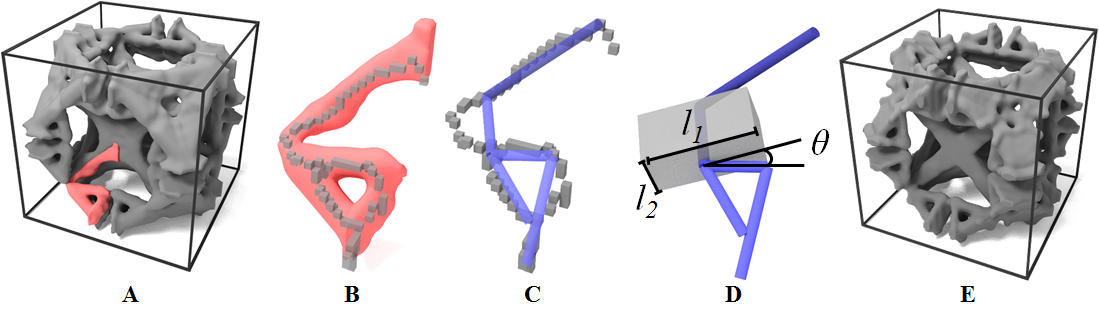
\includegraphics[width=0.95\textwidth]{images/skeletonExtraction.png}
	\caption{Steps for computing a microstructure template from a representative structure. For an input structure (a), we only need to analyze one tetrahedral slice (highlighted in red) of the whole structure due to its cubic symmetric construction. A morphological skeleton is extracted from the portion of the structure (b). The skeleton is a sequence of voxels. They are converted into a graph by connecting neighboring voxels. The graph is simplified (c) by merging paths into single edges while maintaining an error threshold. A cuboid (d) is placed on each edge of the simplified graph. (e) The final structure generated by the template using fitted parameters.}
	\label{fig:skelExtract}
\end{figure}

The final step of our software pipeline computes reduced parameters to facilitate intuitive navigation in the material property space.
Since the templates from the previous step contain tens of parameters that do not directly correspond to material properties, it is still difficult to understand the key design principles.
The reduced parameters allow for direct tuning of each material property.
For a given parametric template, its parameters are fitted to all structures of the corresponding family.
To avoid outliers, microstructures leading to large fitting errors ($>5\%$ voxel difference) are excluded.
Principal component regression (PCR) is then performed on the set of fitted template parameters to find principal directions in the template parameters space.
Varying the parameters in a direction corresponds to moving on the gamut boundary in a certain direction. A reduced parameter is assigned to each direction to control amount of change along that direction.
\subsection{Results and Discussion}
The results of this study focus on elastic material properties: Young's modulus, Poisson's ratio and shear modulus.
The elastic material property gamut is estimated from 15,000 3D cubic-symmetric microstructures at a voxel resolution of $64^3$.
The structures and material parameters are available online~\citep{microDatabase}.
The voxel resolution is a power of 2 because that is necessary to achieve optimal performance of our multigrid FEM simulation.
The specific resolution $64^3$ is chosen because it is sufficient for discovering auxetic structures with a wide range of relative shear modulus while $32^3$ structures cannot achieve comparable complexity or property ranges.
The macroscopic elastic parameter of each microstructure is computed using homogenization theory~\citep{Guedes1990,xia:2015:design} assuming a periodic boundary condition.
Each microstructure consists of a per-voxel binary material assignment. Due to manufacturing limits on minimum feature size,
sensitivity filter~\citep{sigmund:2007} is applied in gamut sampling step to avoid structures with overly thin features.
\begin{figure}
	\centering
	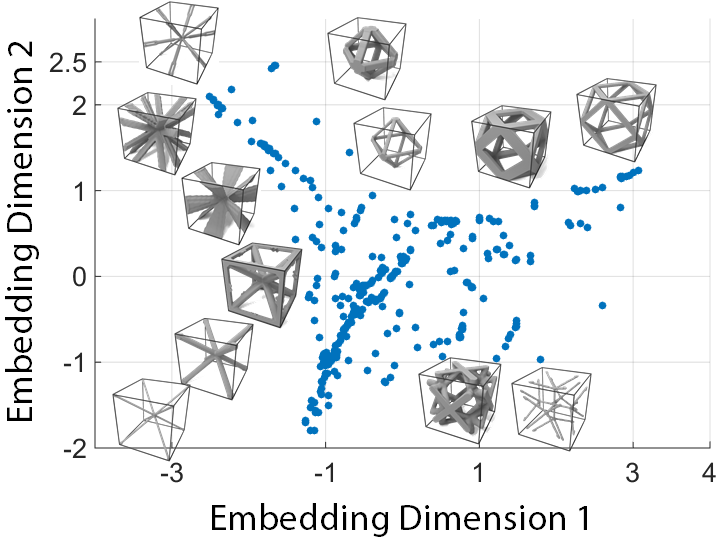
\includegraphics[width=0.5\columnwidth]{images/pprFamily.png}
	\caption{Structures with large Poisson's ratios ($\nu>0.3$). The embedding is computed using Isomap with 3 dimensions while the plot shows the 2D projection of the embedding. Structures with a positive Poisson's ratio have relatively simple topologies. Most structures are controlled by a single beam reflected according to cubic symmetry.}
	\label{fig:pprfamilies}
\end{figure}
\begin{figure}
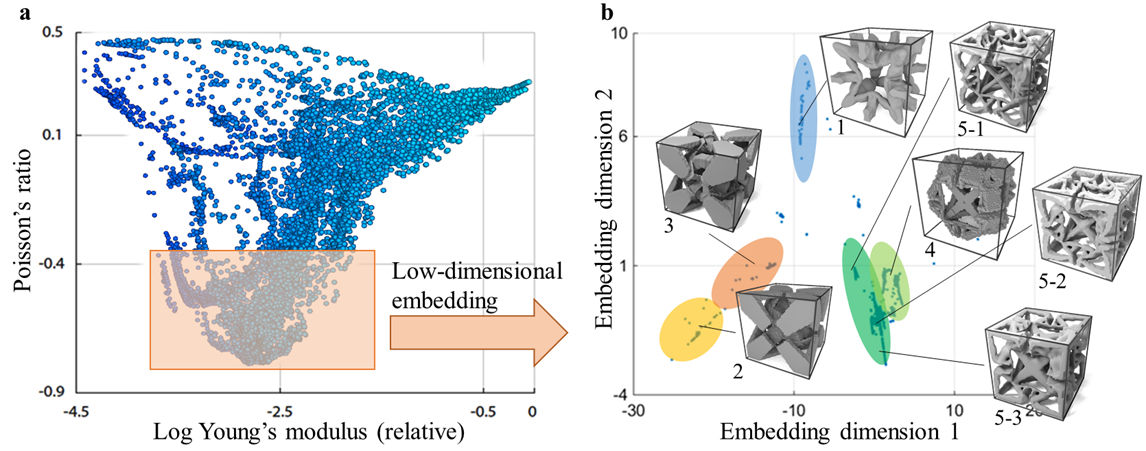
\includegraphics[width=0.95\columnwidth]{images/fiveFamilies.png}
\caption{Five microstructure families identified by nonlinear dimensionality reduction (NLDR). Structures with similar properties in the gamut (a) are selected to study their commonalities. We focused on structures with negative Poisson's ratio (auxetics) since they exhibit more complex structures. Auxetic families are identified in the embedding space numbered from 1 to 5 (b). Families with similar topologies are located closer in the embedding space. Three example structures from family 5 show underlying connection between seemingly distinct structures through gradual morphing of shape.}
\label{fig:families}
\end{figure}
Here we focus on analysis of auxetic structures since families with positive Poisson's ratios are relatively simple (Figure~\ref{fig:pprfamilies}). Five families with significant number of members (Figure~\ref{fig:families}) are discovered using three Isomap embedding dimensions. We confirmed that Isomap associates seemingly distant structures through intermediate structures. For example, structure 5-1 and 5-3 from family 5 have very different beam thicknesses resulting in large geometric distance. However, the embedding reveals that there is a sequence of structures such as 5-2 that make the connection between them.

Three structures with different material properties from each family are printed to verify simulation accuracy.
All structures are printed using an EOS SLS printer with elastic material PEBA2301.
The printer required a minimum feature size of $0.9mm$ for wire diameters and $0.8mm$ for wall thicknesses.
To satisfy the printing constraints, each cell is scaled to a side length of $2.54mm$.
Simpler structures from Template 1-3 are printed using a 2x2x2 grid arrangement while more complex families are printed using a 3x3x1 arrangement to allow support material to escape.
The base printing material is measured using an Instron 5944 with tensile tests instead of compression tests since a solid block of base material is too stiff for our equipment.
The Poisson’s ratio is measured using a video camera fixed on the test machine (Figure~\ref{fig:measure}).
Even though all samples are printed using the same printer and the same materials, the Young’s modulus of the prints is highly variable.
More specifically, the stiffest sample has a Young’s modulus which is twice as high as the one of the softest samples.
On the other hand, the Poisson’s ratio of the base print material is measured to be $0.34$ and has a much lower variance of $0.02$ in the sample set.
The 3D structures are measured using a compression test at a speed of $2mm/min$ with $6mm$ maximum strain.
The compression plates are lubricated with oil to reduce friction.
Significant variance in Poisson’s ratio is observed due to several factors in manufacturing and measurement.
An additional challenge is that the printer does not reliably reproduce the geometry specified by input files.
In practice, the printed models are thickened by $0.1-0.4mm$, which is significant compared to the thinnest feature size in our microstructures.
This stiffens the joints and reduces Poisson’s ratios.
The effect is exacerbated by incomplete support removal.
The support material is the same as the print material in powder form, which sticks to the print easily especially around hard-to-reach internal corners.
We believe that the discrepancy can be reduced in the future by using more precise printing technologies with soluble support material.
\begin{figure}
	\centering
	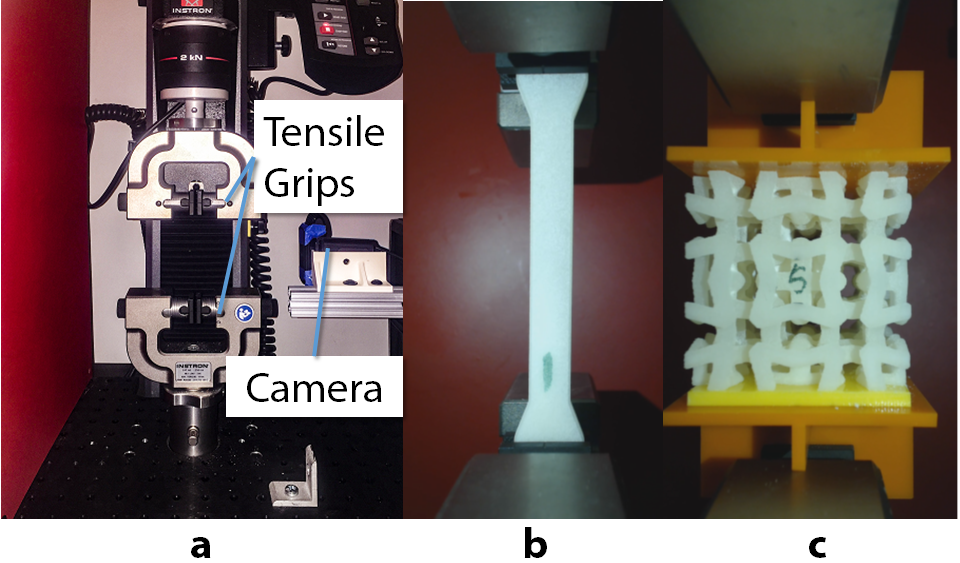
\includegraphics[width=0.5\columnwidth]{images/measure.png}
	\caption{Test apparatus (a) for measuring Young’s modulus and Poisson’s ratio using tensile (b) and compression (c) tests. The Poisson’s ratio is calculated using vertical displacements and horizontal displacements. The vertical displacement is read from both the tensile test machine and the camera for redundancy. The horizontal displacement is measured using the camera only.}
	\label{fig:measure}
\end{figure}
\begin{figure}
	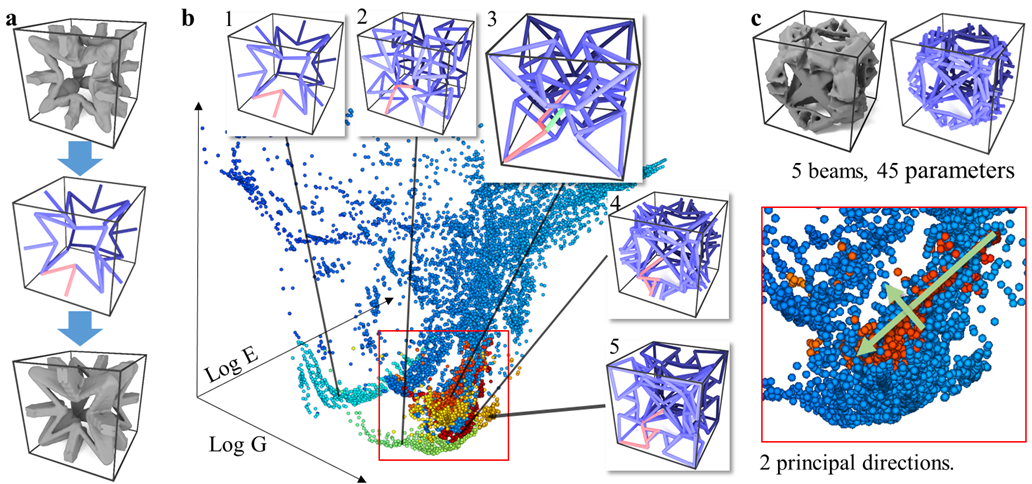
\includegraphics[width=\columnwidth]{images/mTemplates.png}
	\caption{Sampled coverage of microstructure templates in the gamut. (a) Extracting a skeleton (middle) from a representative structure (top). The skeleton represents the topology of the structure. A beam network is derived from the skeleton by placing a cuboid on each edge of the skeleton. Since we enforce cubic symmetry, the beams in a single tetrahedron determine the entire beam network. A template can generate a new structure (bottom) that approximates the original structure. (b) Coverage of each template in the material property space. (c) Reducing template parameter dimensions with principal component regression. The first two reduced parameters approximately correspond to varying the Young's modulus and Poisson's ratio of a structure. }
	\label{fig:mTemplates}
\end{figure}
For each of the five families, a parametric template is automatically constructed. The initial topology of a template is extracted from the morphological skeleton of a representative structure (Figure~\ref{fig:mTemplates}b). While the topologies are visually complex, they are generated by mirroring a small number of beams (highlighted in red) reflected according to cubic symmetry (Supplementary Table 2). The most complex template 5 contains only 6 control beams. The five families cover similar ranges of Young's modulus and Poisson's ratio. However, they span different ranges of shear modulus. Inspired by classical linear elasticity theory, we compare the shear modulus ratio defined as
\[
G'=\frac{2G(1+\nu)}{E},
\]
where $G$ is shear modulus, $E$ is Young's modulus and $\nu$ is Poisson's ratio. For traditional isotropic materials, the theoretical ratio is one. A low ratio indicates low resistance to shear deformation. For auxetic materials, lower ratios are much easier to obtain than higher ones. Even with foam structures assumed to be isotropic, experimental data from previous work indicates that the ratio is less than one~\citep{roh2013failure}.
\begin{figure}
	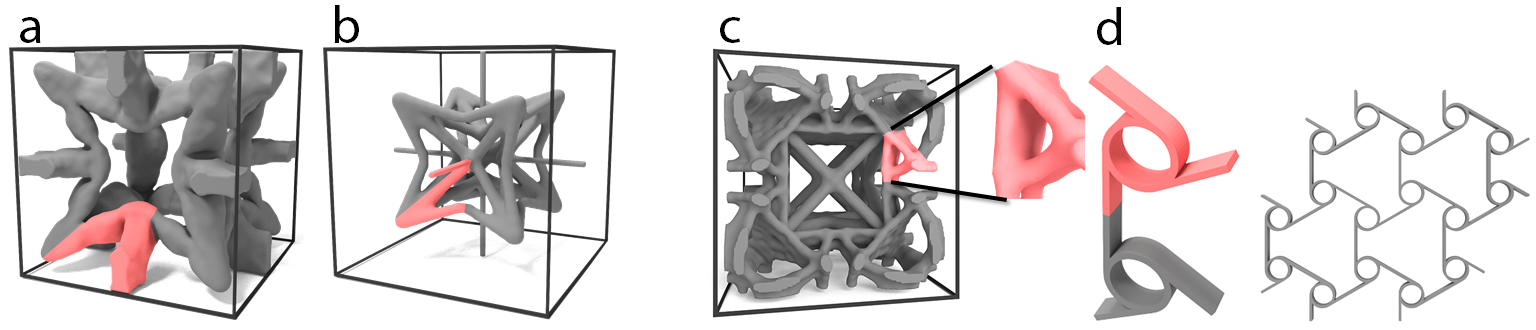
\includegraphics[width=0.9\columnwidth]{images/similarShape.png}
	\caption{Microstructures that resemble designs from previous works. (a) A reentrant structure in our database similar to the conceptual sketch (b) proposed by ~\citet{lakes1987foam}. Both structures have very low shear modulus ratio (0.05-0.15). Our structure is simpler with only two control beams reflected by cubic symmetry while (b) has three beams (highlighted in red). (c) The rotating triangle mechanisms resembles 2D chiral structures~\citep{prall1997properties}. (d) An anti-trichiral lattice~\citep{alderson2010elastic} has unit nodes most similar to our rotating triangle joints (highlighted in red).}
	\label{fig:similarShape}
\end{figure}
Template 1 resembles the conceptual sketch by~\citet{lakes1987foam} and belongs to the reentrant class of geometry. The difference is that our template has only two beams mirrored by cubic symmetry while Lakes' sketch contains three (Figure~\ref{fig:similarShape}). It is the simplest auxetic template that we identified, as our microstructure database does not contain any single-beam auxetic structure. The shear modulus ratio of this family falls in the range between 0.07 and 0.24, which is the lowest among all five families. Templates 2 and 3 are similar to each other and differ by a diagonal beam in the face center (highlighted in green in template 3). Since their geometric difference is small, they are adjacent in the Isomap embedding space. The central beam is responsible for increasing the shear modulus of the structures. For structures with $\nu$ around -0.5, the additional beam increases the maximum shear modulus ratio from 0.34 to 0.90. Templates 4 and 5 also differ by a single beam. Even the most complex template 5 is optimized from a simple cube frame through our continuous optimization step. The additional beam in template 5 makes the family stiffer overall compared to Template 4. Both families can achieve shear modulus ratio greater 1 for $\nu<-0.5$.

For each family, principal directions of template parameters are extracted using PCR. The templates and reduced parameters are included with the report. Two significant directions correspond to change in Young's modulus and shear modulus are kept for tuning structures. These directions reveal that for families 2 and 3, the thickness of the slanted column (Figure~\ref{fig:auxeticMech}a highlighted in red) is crucial for Poisson's ratio where the Poisson's ratio increases quickly with increasing beam thickness.
For families 4 and 5, the thickness of the rotating triangle affects the tradeoff between Young's modulus and shear modulus (Figure~\ref{fig:paramReduction}).
\begin{figure}
	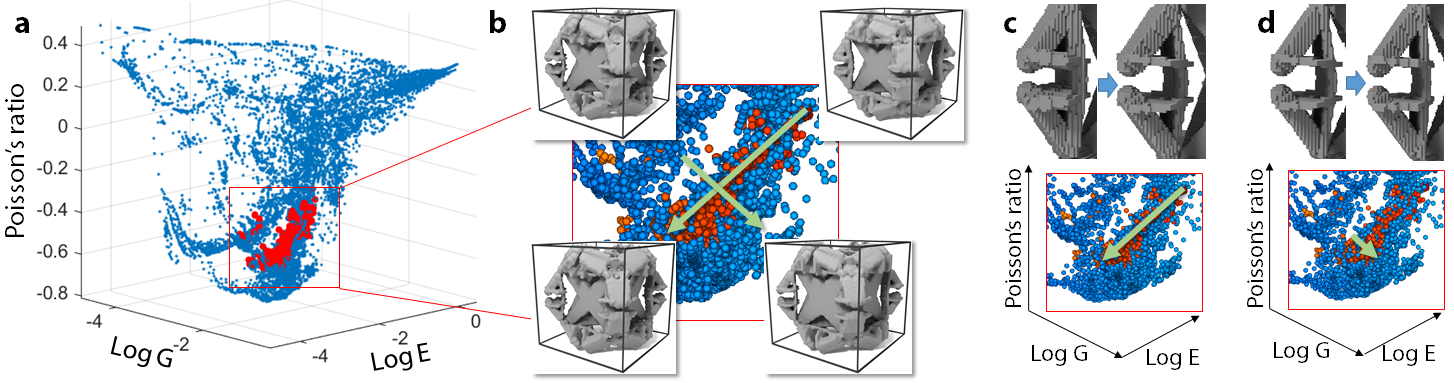
\includegraphics[width=\columnwidth]{images/paramReduction.png}
	\caption{Reduced parameters for Family 4. The distribution of the parameters corresponding to Family 4 is shown as red points in (a). The two principal directions are shown as green arrows in (b). The first direction reduces the Young's modulus and Poisson's ratio by decreasing the joint thickness (c). The second direction increases the shear modulus by slightly rotating the triangle joints outward (d).}
	\label{fig:paramReduction}
\end{figure}
While our cuboid-based templates are very simple, they are sufficient for replicating the auxetic behavior of the corresponding families.
We validated the auxetic properties of the fitted microstructures using simulation.
New structures are generated by varying template parameters.
300 new structures are sampled from each family along two PCR coordinate directions.
The coverage of the templates in the microstructure gamut (Figure~\ref{fig:mTemplates}b) shows that the templates can generate microstructures on the gamut boundary.

So far all of our simulations are carried out assuming linear elasticity, which is only accurate for infinitesimal deformations. We also make the common assumption that there is no self-collision. This assumption also imposes a limit on the maximum compressive strain we can apply to our structures before self-collision occurs. Representative structures from Families 4 and 5 have the lowest limit at $7\%$ compressive strain.
In practice, non-linear deformations such as bending and rotation are prevalent in our auxetic structures. Such deformations can cause linear elasticity to incorrectly predict significant volume expansion of rotated parts (up to $20\%$ percent in our test cases).
Thus, we tested our structures using a nonlinear material model to understand their behavior under large deformations.
We simulated nonlinear deformation behavior using Neo-Hookean material model.
At maximum allowed strain of $7\%$, linear elasticity and Neo-Hookean model still has acceptable agreement with an average error of $16\%$ in computed Poisson's ratio. In addition to simulation, we also printed three example structures from each family with varying Young's modulus and material ratio. Our structures demonstrated consistent auxetic behavior (Supplementary Video 3) even though they are optimized with linear elasticity assumption.
Our structures do not rely on structural instability~\citep{bertoldi2010negative} for auxetic behavior and shrinks uniformly as load increases.
This means that their deformations consistently follow the same pattern for different trials.

\begin{figure}
	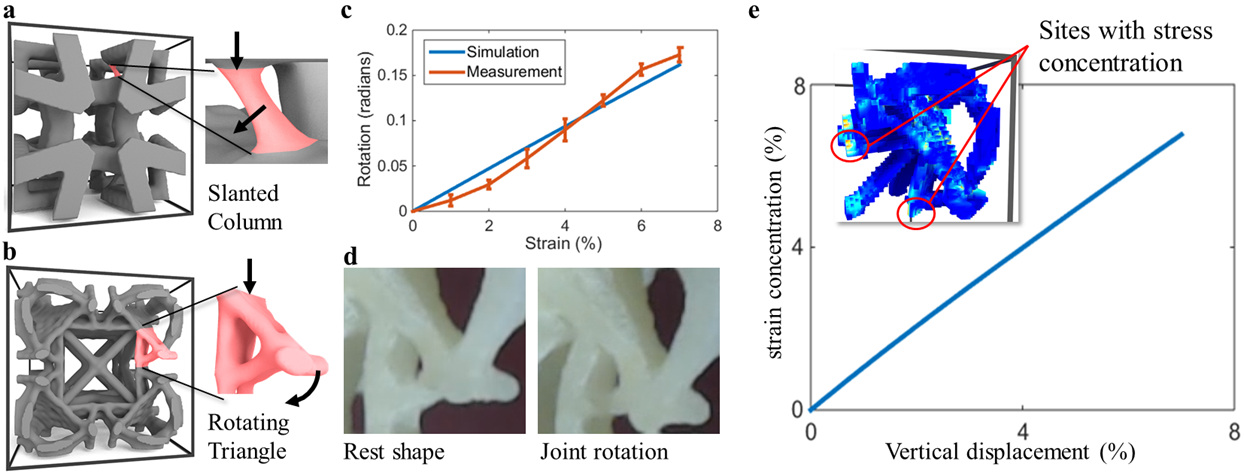
\includegraphics[width=\columnwidth]{images/auxeticMech.png}
	\caption{Discovered auxetic mechanisms. Two mechanisms capable of producing auxetic behavior are discovered from our microstructure families. The slanted column (a) transforms vertical stress into horizontal displacement. The rotating triangle mechanism (b) pulls the outer tip of the joint towards the center of the structure, reducing the macroscopic volume. (c) The relationship between vertical strain and rotation of the triangle joint. The rotation is observed in printed samples under vertical load (d). Stress is concentrated at the lower end of the triangle joint (e).}
	\label{fig:auxeticMech}
\end{figure}
Our process automatically discovered two types of auxetic mechanisms: slanted columns and rotating triangles (Figure~\ref{fig:auxeticMech}). The slanted column mechanism transforms vertical compression to horizontal motions. The rotating triangles transform vertical compression into a winding deformation that pulls the right end of the mechanism towards the center of the microstructure.
Their motions are shown in supplementary video S3.
While rotating triangles bear resemblance to existing 2D structures~\citep{alderson2010elastic} known as chiral structures (Supplementary Fig. 6d), its extension to 3D cubic structure with large shear modulus has never before been constructed. Additionally, the entire mechanism is discovered entirely automatically without imposing any artificial design restrictions---all microstructures are built from voxels. To inspire future applications of these mechanisms, we report the loading behavior of the mechanisms. These auxetic mechanisms are the most active parts in the microstructures. They act like joints that connect the more rigid scaffolding in microstructures. Because of this, they undergo the most deformation and concentrate a large amount of stress. For the rotating triangles, the stress is concentrated on the connections around the triangle. We computed the maximum principal strain in the structure with respect to the vertical compressive loading to provide insights into the strength of the block.
At the maximal compressive loading $(7\%)$, the maximum principal strain in the structure is $7\%$. Calculation using a reported Young's modulus of $80MPa$ yields a von Mises stress of $6.72MPa$ (Fig. 4e) while our print material has a reported strength of $8.5MPa$. The printed structures are approaching the strength limit under the load. Since the available material is relatively weak even compared to common materials such as ABS plastics and rubber, we believe that structural strength can be improved significantly with future manufacturing materials.

We have shown a computational method that combines discrete sampling, continuous optimization and dimensionality reduction methods for automatic discovery of new microstructure families and mechanisms that would have been challenging to design manually.
The discovered structures are suitable for manufacturing as they avoid thin features and distribute deformation over beams instead. They also span a wide range of shear moduli, allowing engineers to balance between different macroscopic properties. While our case study focuses on elastic material properties, the technique may be applied to other physical properties whenever predictive simulation exists. Our computational pipeline paves the way to discovery of structures that balance mechanical, thermal, optical, acoustic and electromagnetic properties. Moreover, it advances the understanding of underlying mechanisms that are crucial to extremal properties.
